\chapter{Objemová grafika}\label{chap:grafika}
Vďaka pokroku vo vývoji hardvéru sa revolučné prístupy k počítačovej grafike postupne stávajú realitou, a to aj pre bežného majiteľa počítača. Dobrým ilustratívnym príkladom pre nás môže byť rastrová grafika, ktorá sa objavila v období, kedy hardvérové inovácie dopomohli k reálnemu presunu z matematicky reprezantovanej vektorovej grafiky k pamäťovo náročnejšej rastrovej grafike.
Podobným príkladom je aj objemová grafika, ktorej rozvoj opísali vo svojom článku v roku 1993
Kaufman, Cohen a Yagel \cite{VolumeGraphics}.

Objemová grafika teda predstavuje prechod od takzvanej povrchovej grafiky, ktorá objekty reprezentuje pomocou spojitých primitív ako sú polygóny alebo free-form povrchy, k reprezentácii objektu pomocou diskrétnych objemových štruktúr \cite{Winter}, ktorých základná dátová jednotka je voxel opísaná nižšie v tejto kapitole.
Taktiež môžme povedať, že objemová grafika je významným poľom počítačovej grafiky a je 3D analógiou rastrovej grafiky. Jej uplatnenie sa našlo nielen vo vizualizácii rôznorodých vedeckých dát, ale aj v komerčnom využití ako napríklad herné enginy, animácie alebo umenie.

Avšak objemová grafika naďalej zostáva menšinou na poli počítačovej grafiky, pretože jednou z hlavných prekážok jej širšieho použitia je fakt, že niektoré z fundamentálnych operácií ešte potrebujú vylepšenie teoretických základov a taktiež objemová grafika, na rozdiel od tej povrchovej, nemá podporu grafických akcelerátorov. Na druhej strane sa mnohé z techník objemovej grafiky stali populárnymi v radoch
vývojárov najrôznejších grafických aplikácií, pretože objavili nesporné výhody tohto
prístupu v určitých oblastiach.
\cite{Tomas}

\section{Objemové dáta}
Ako bolo spomenuté vyššie, najbežnejším prístupom k reprezantácii objektov v trojrozmernom priestore je
povrchová reprezentácia objektov pomocou dvojrozmerných primitív. Tento prístup je však v mnohých prípadoch nedostačujúci, pretože sa takto strácajú informácie o vnútornej štruktúre 3D telies.
Nastolený problém riešia objemové dáta, ktoré tieto informácie obsahujú. Vďaka tejto vlastnosti je objemová reprezentácia vhodný kandidát pre medicínske, geologické, biologické, archeologické a iné vedecké dáta získané napríklad v prípade medicíny z tomografu.\cite{RealTime} V hernom priemysle je takáto reprezentácia vhodná na detajlnú deštrukciu okolitého prostredia alebo je taktiež vhodná na modelovanie amorfných objektov ako sú napríklad oblaky, dym a podobne. 

Vizualizácia objemových dát sa markantne líši od vizualizácie povrchových telies, keďže objemové dáta neobsahujú žiadnu explicitnú ifnormáciu o povrchu a taktiež je nevyhnutne potrebné nejako nahliadnuť do vnútra objektu. Cieľom vizualizácie objemových dát je teda vytvoriť mechanizmus, ktorý nám umožní extrahovať zmysluplné infromácie z objemových dát pomocou ich reprezentácie, manipulácie a renderingu.

Objemové dáta sa najčastejšie uchovávajú v trojrozmernom poli a teda sú zvyčajne reprezentované ako štvorica $(x,y,z,v)$, kde $(x,y,z)$ sú poloha v 3D priestore $v$ je $value$, teda hodnota danej objemovej jednotky, čo môže byť napríklad $0$ alebo $1$, kde hodnota $0$ indikuje prázdne miesto a $1$ indikuje objekt. Táto hodnota môže byť aj komplexnejšia informácia, ako napríklad farba, hustota, tlak alebo vektor zrýchlenia v danej polohe $(x,y,z)$.
\cite{VolumeGraphics} Alternatívne dátové štruktúry na uchovávanie a manipuláciu objemových dát sú napríklad octrees, voxelové riedke matice, '\textit{voxel runs}' alebo nepravideľné mriežky. Tieto štruktúry sú zvyčajne vhodné na dobrý manažment pamäťových zdrojov alebo majú iné výhody napríklad v detekcii kolízií.
\section{Voxel}
Elementárnou jednotkou objemovej grafiky je voxel. Je priamou 3D analógiou pre jednotku dvojrozmerného priestoru v pravidelnej mriežke, teda pixel. Podobne ako slovo pixel (picture element) slovo voxel je len skratkou pre zložitejšie pomenovanie volume element. Ako bolo dostatočne opísané v predchádzajúcej kapitole, každý voxel okrem svojej polohy v priestore obsahuje aj nejakú merateľnú hodnotu. 

Analógia, pre voxeli s pixelmi, sa zachováva aj pri uchovávaní voxelov v pravidelnej mriežke. Teda zatiaľ čo sú pixely uchovávané vo \textit{frame buffery}, voxely sa uchovávajú vo \textit{volume buffery} alebo tiež nazývanom \textit{3D raster}, či \textit{objemový frame buffer}.

Zadefinovaním tohto pojmu môžeme teraz hovoriť o voxelovom priestore alebo tiež o voxelovej grafike.

\section{Porovnanie s povrchovou grafikou}
Spomenuli sme už majoritné rozdiely medzi povrchovou a voxelovou grafikou, ktoré priamo vyplývajú z ich pomenovania. V tejto časti sa teda zameriam na porovnanie týchto dvoch prístupov detajlnejšie s dôrazom na výhody a nevýhody objemovej grafiky oproti povrchovej.

\subsection{Nevýhody}
Pri reprezentácii scény sú voxely usporiadané v pravidelnej trojrozmernej mriežke, teda hovoríme o diskrétnom priestore. Tento fakt spôsobuje mnohé komplikácie analogické ku komplikáciám v rastrovej grafike.

Jedným z hlavných problémov je poškodenie, teda modifikácia alebo strata informácii o objekte pri jeho transformácii. Pri rotácii objektu o uhol \begin{math} \alpha \neq k\frac{\pi}{2}, k \in \mathbb{Z} \end{math}  vznikajú diery. Podobne aj pri škálovaní o koeficient \begin{math}k > 1\end{math} je očakávaný vznik dier a pri škálovaní o koeficient \begin{math}k < 1\end{math} nastáva strata informácie. Keďže tieto problémy súvisia taktiež s rastrovou grafikou, vzniklo dostačujúce množstvo techník (supersampling, bilineárna interpolácia a pod.) ako tento problém riešiť s viac-menej uspokojivým výsledkom.

Keďže voxelové objekty sú získavané vzorkovaním, nevyhnutne vznikajú artefakty. Tie vidieť najmä pri bližšom zazoomovani na danú oblasť. Teda môžme povedať, že voxelové objekty sú nepresné a sú len diskrétnou aproximáciou pôvodných objektov, kde hustota 3D mriežky určuje ich presnosť.

Prítomnosť objemu vo voxelových objektoch spôsobuje ďalší problém charakteristický pre voxelovú grafiku, a tým je pamäťová a procesová náročnosť. Pomerne malý objekt s rozmermi \begin{math}512^{3}\end{math} pozostáva z približne \begin{math}1.35\cdot 10^{8}\end{math} voxelov. Ak by sme každý voxel reprezentovali iba jediným bytom, tak pre takýto objekt by bolo potrebné 128MB pmäte. Tieto veľké objemy priamo spôsobujú, že voxelová grafika je náročná aj na processing. Príkladom môže byť rendering, transformácie alebo aj voxelizácia.

\subsection{Výhody}
Okrem niekoľkokrát spomenutého faktu, že objemová grafika obsahuje aj informácie o vnútornej štruktúre objektov, nám voxelový priestor ponúka ďalšie nesporné benefity.

Jedným z nich je jednoduchosť rôznych operácií, ako je napríklad sekanie, orezávanie alebo aj booleanovské operácie medzi objektami. Zatiaľ čo pri povrchovej grafike sú tieto operácie pomerne komplexné a zložito implementovateľné, vo voxelovej grafike sa tieto operácie posúvajú až na úroveň voxelov a teda predstavujú triviálny problém. Ak si zvolíme Constructive Solid Geometry (CSG) ako modelovaciu paradigmu, tak je táto vlastnosť voxelových objektov ohromnou výhodou.

Ďalšou výhodou je, že voxelová grafika nie je citlivá na členitosť objektov. Pri väčšej členitosti objektu v povrchovej grafike narastá počet polygónov a teda aj požiadavky na zdroje, zatiaľ čo voxelový objekt si svoju zložitosť zachováva konštantnú. Podobne aj pri mapovaní textúr (znázornené na obrázku \ref{tank}) má objemová grafika výhodu, pretože na voxelový objekt stačí namapovať textúru iba raz, kedy sa vypočíta farba pre každý voxel a v ňom sa aj naďalej uchováva, zatial čo mapovanie textúr na polygónový respektíve povrchový objekt sa vykonáva zvyčajne až na konci renderovacej pipeline.

\begin{figure}[ht!]
	\centering
	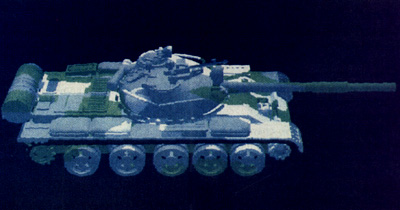
\includegraphics[width=90mm]{tank.jpg}
	\caption[Voxelový tank s namapovanou textúrou]{Voxelový tank s namapovanou textúrou}
	\label{tank}
\end{figure}

\eject

\section{Komerčné využitie}
Technologický pokrok umožnil, že objemovú grafiku je možné realizovať aj na bežnom-širokodostupnom hardvéri. Toto otvorilo dvierka pre komerčnú sféru technologického rozvoja, a tak sa voxely objavujú nielen ako pomôcka pre zobrazenie pseudonáhodných čísel v teoretickej informatike, ale aj ako stavebné častice herného prostredia, či nástroj na tvorbu detajlných skulptúr.

\subsection{Herný priemysel}
Prvou firmou, ktorá sa odvážila využiť voxely ako stavebný prvok pre svoj herný engine bola spoločnosť \textit{NovaLogic} v roku 1992 v hre \textit{Comanche: Maximum Overkill} \cite{VoxelGames} . Išlo o letecký simulátor, ktorý voxelovú technológiu použil na vytvorenie detajlného vykreslenia okolitého terénu, aký je na obrázku \ref{comanche}. V roku 1996 táto spoločnosť za podobným účelom vytvorila populárnu bojovú hru \textit{Delta Force}.

V roku 2000 začal pracovať programátor Ken Silverman spolu s Tomom Dobrowolskym na svojom prvom plne voxelovom hernom engine s názvom \textit{Voxlap}. \cite{Voxlap} Ten je teraz spolu so zdrojovými kódmi voľne dostupný na svojej oficiálnej stránke a ponúka vykreslovanie voxelového priestoru v pomerne dobrom rozlíšení.

Hra, ktorá najviac spopularizovala voxelovú grafiku vo svojej upravenej podobe, vznikla v roku 2010 s názvom \textit{Minecraft}. Princípom hry je dolovať v hlbokom podzemí bloky rôznych stavebných materálov. Takýmto spôsobom hra využíva najdôležitejšiu vlastnosť voxelovej grafiky, ktorou je uchovanie infromácie o vnútornom obsahu objektu. 

\begin{figure}[ht!]
	\centering
	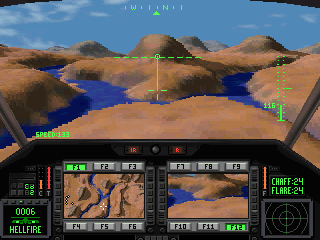
\includegraphics[width=90mm]{comanche.png}
	\caption[Ukážka voxelového terénu z hry Comanche: Maximum Overkill]{Ukážka voxelového terénu z hry \textit{Comanche: Maximum Overkill}}
	\label{comanche}
\end{figure}

\subsection{Umenie}
Informatika a obzvlášť počítačová grafika je natoľko ohromujúca, že svojím vplyvom zasahuje i do umenia. Nie je teda prekvapením, že voxely si našli svoje miesto aj medzi umelcami. 

Dobrým príkladom je napríklad aj digitálne sochárstvo (\textit{Voxel sculpting}). To umožňuje pre umelca slobodu modelovania digitálnych sôch bez akýchkoľvek topologických obmedzení a vytvárať komplexné detajly takmer z ničoho. Táto sloboda je dosiahnutá vďaka tomu, že úprava sôch nie je založená na deformácii povrchu, ale na vytváraní a vyplňovaní objemu. \cite{Sculpting}

Voxelart je ďalším smerom digitálneho umenia, ktoré je 3D obnožou pre pixelart. Na rozdiel od digitálneho sochárstva vo voxelarte sa kladie dôraz na každý vložený voxel, ktorý dotvára celkový dojem z diela. Zvyčajne takéto výtvory bývajú aj omnoho jednoduchšie, keďže ich tvorba je náročnejšia.

Svojou jedinečnosťou zaujali voxely aj animátorov a na internete je možnosť nájsť pomerne veľké množstvo zaujímavých kockatých animácií.